Escolhemos como cenário de teste uma sala com alguns obstáculos, conforme mostrado na Figura ~\ref{fig:nav}. Fizemos então um nó (em C++) que publica dois \textit{goals} para o \verb|move_base|, no qual o caminho mais próximo seria colidindo em objetos do ambiente. Conduzimos os testes e chegamos às seguintes conclusões:
\begin{compactitem}
\item Os obstáculos, além de uma área em volta deles, eram corretamente evitados pelo robô, que fazia o máximo para gerar um caminho seguro que chegasse ao seu destino. 
\item O robô atualiza frequentemente seu caminho, buscando melhores alternativas conforme vai melhor reconhecendo o ambiente.
\item Os mapas de custo global e local apresentavam dados condizentes entre si e também condizentes com o que era mostrado no mapa criado pelo \verb|gmapping|. Na Figura \ref{fig:nav}, o que se vê é o mapa local, já que ele está quase perfeitamente encaixado com o mapa global, que está por baixo. Se olharmos no canto superior da imagem, podemos ver uma pequena porção do mapa global, da mesma coloração do local, mas bem mais claro. Não é possível perceber a diferença entre o local e o global na Figura \ref{fig:costmap} e na Figura \ref{fig:nav} já que os dois estão praticamente perfeitamente sobrepostos. Este é o resultado desejado, sendo que erro na sobreposição dos mapas implica em erros na navegação.
\item Devido aos erros da odometria, o mapa de custo local 'desliza' sobre o mapa de custo global. Após algum tempo, o \verb|gmapping| publica uma nova transformação entre os \textit{frames} do mapa e do \verb|odom| e corrigia esse erro, realinhando os mapas.
\item Nos testes, vimos também que o ângulo de visualização bastante fechado do Kinect limita muito o seu funcionamento e faz o robô ter muita incerteza quanto ao ambiente. Esse sensor se mostrou inferior aos sensores scanners a laser de distância para essa aplicação.
\end{compactitem} 

\begin{figure}[H]
\centering
  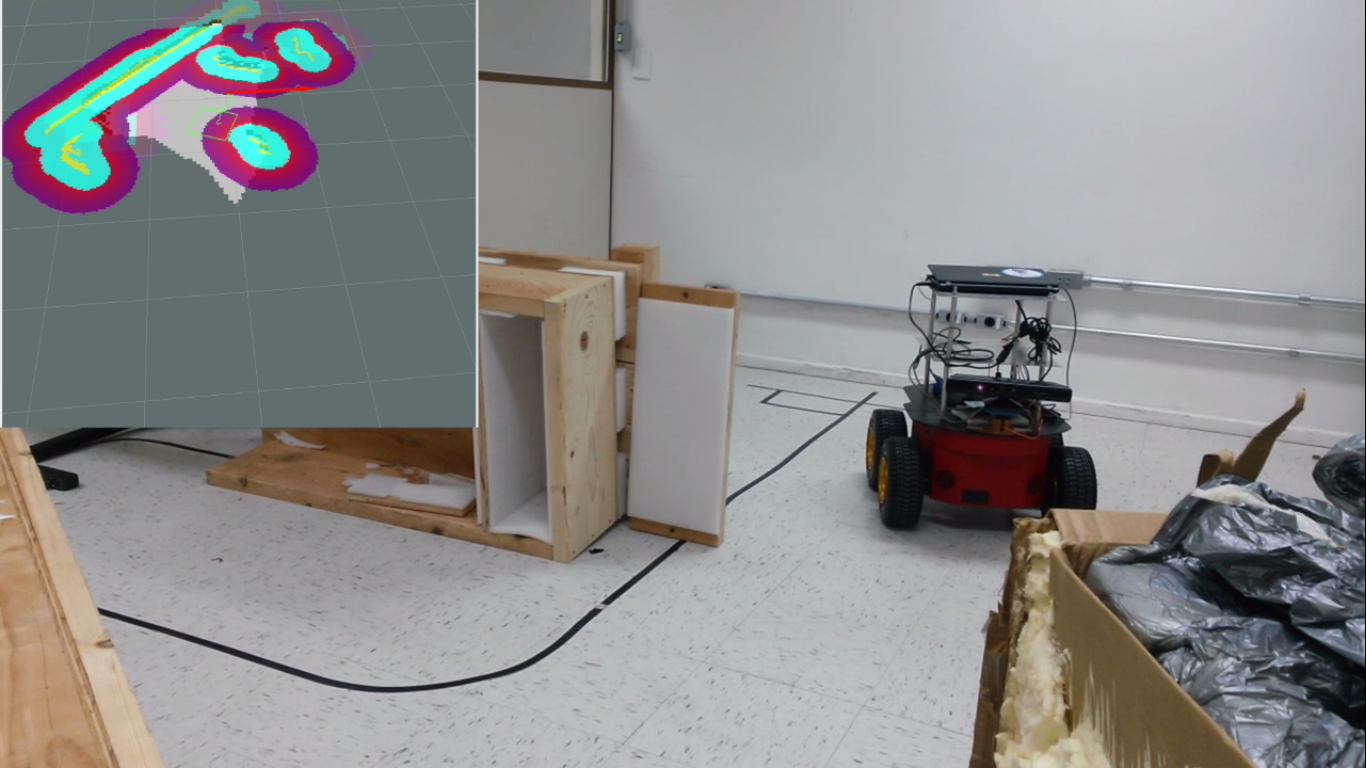
\includegraphics[width=12cm]{images/nav.png} 
\caption{\small{Robô móvel Pioneer 3-AT navegando no cenário de testes. No canto esquerdo superior é possível ver o mapa de custo gerado, além do \textit{footprint} do robô e da trajetória atual.}}
\label{fig:nav}
\end{figure}

\begin{figure}[H]
\centering
  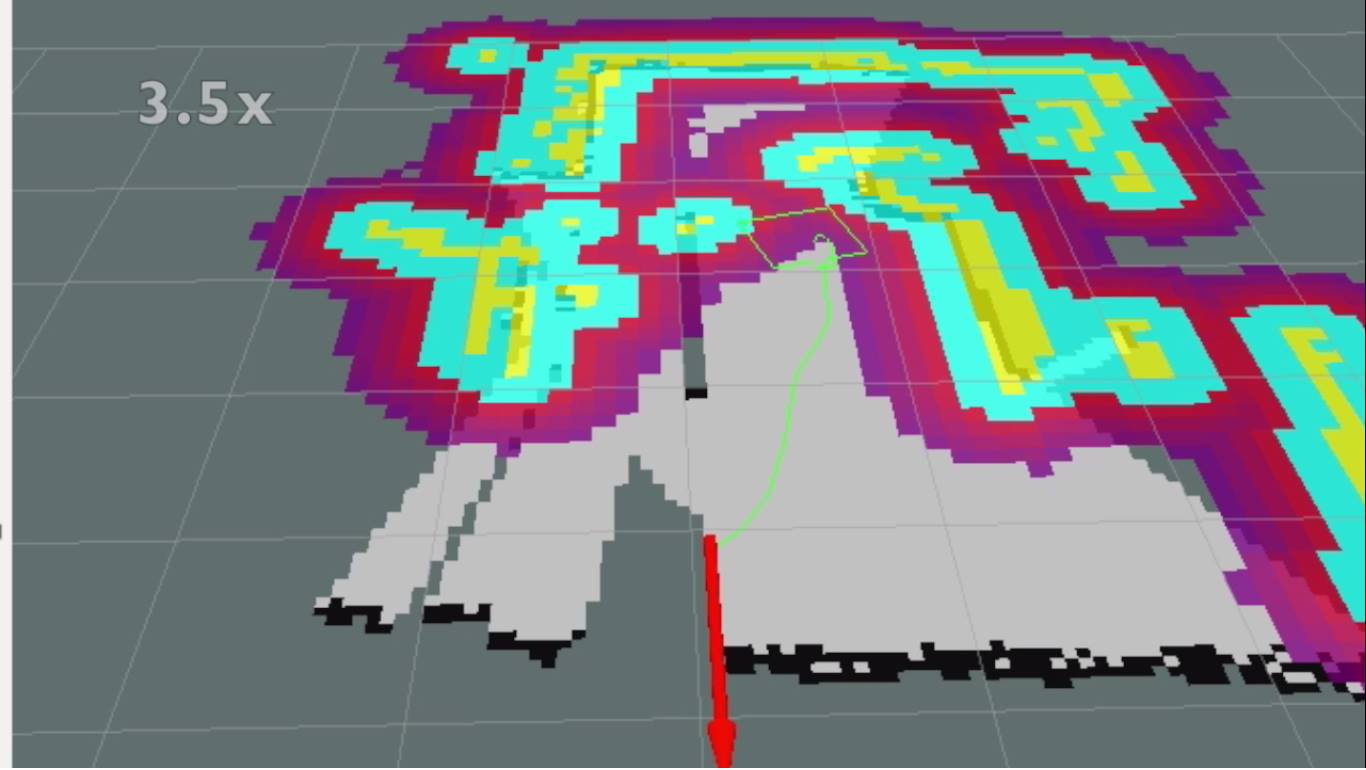
\includegraphics[width=12cm]{images/MapaCusto.png} 
\caption{\small{Imagem detalhada de um exemplo de mapa de custo em um cenário de teste. Os mapas de custo local e global estão perfeitamente sobrepostos na imagem, sendo este um resultado ótimo. A linha preta delimita áreas de mudança de mapa local para mapa global, sendo o global o maior dos dois.}}
\label{fig:costmap}
\end{figure} 